\section{Rectangle networks and boundary partition comparisons}
\label{sec:rectangles}

This section has two outputs. Proposition~\ref{prop:rectangle-rsw}
gives rectangle crossing bounds when the two crossing electrodes are
wired separately and the remaining boundary is ordinary.
Lemmas~\ref{lem:one-sided-density} and~\ref{lem:separate-caps} compare
partition-function gains from caps on separate accessible boundary arcs.
The first output supplies local connections; the second controls how
those connections and local laws change when a region is attached to
its exterior. Both use only the finite comparisons of
Section~\ref{sec:pressure} and planar geometry.

The rectangle argument is by contradiction. Near-square bounds and
interlacing will turn a vanishing crossing probability into many
almost-certain crossings of winding corridors. A geometric packing
bound rules out that conclusion. We prove the packing bound, use it
to establish Proposition~\ref{prop:rectangle-rsw}, and then turn to
the boundary partition comparisons.

Throughout, $0<q<1$ is fixed, $v=\sqrt q$, and $t=q^{-1}$.  For a finite
graph $G$ and two disjoint nonempty vertex sets $A,B$, write
\[
 g_G(A,B)=\PP_{G/(A,B)}(A\leftrightarrow B),
\]
where $G/(A,B)$ means separate contraction of $A$ and $B$.
Unless explicitly specified, the graphs used below consist of physical
edges and have no other identifications. The tested event is connection
of the two quotient vertices. In that setting, this two-wire law is
equivalent to the existence of an actual open path from $A$ to $B$ in
$G$. With additional wires, that equivalence must be checked afresh.

An accessible boundary interval will mean an interval on the boundary of
a topological disk containing its marked vertices in their boundary order,
with all physical-edge incidences on the disk side.  Equivalently, narrow
outward prolongations put each marked vertex in a single boundary slot
with an inward physical-edge fan.  Wires on such an interval can be drawn
as links in a narrow exterior cap.  A noncrossing partition of an interval
means a partition realizable by nonintersecting links in that cap.

\subsection{The permitted finite comparisons}

We first record precisely which consequences of Section~\ref{sec:pressure}
will be used.  Adding vertices to a tested terminal does not decrease $g$:
realize the added contractions by edges incident to that terminal and
apply Lemma~\ref{lem:adjacent-rayleigh} against a connection test edge.
Moreover, Lemma~\ref{lem:rooted} gives
\begin{equation}
 g_G(A,B_1\cup B_2)\le g_G(A,B_1)+g_G(A,B_2)
 \label{rect:subadditivity}
\end{equation}
whenever the electrodes are disjoint from $A$.  Indeed the three
quantities are hitting probabilities under the same rooted-multiset law
on $G/A$.  The analogous inequality holds in the first terminal.

There is also a restricted geometric extension comparison.  To test
connection of two exposed terminals, draw an auxiliary edge between them
in the exterior face and take its odds to zero.  Its partition-function
derivative is
\[
 \PP(\text{connection})+q^{-1}\PP(\text{separation}).
\]
Thus the cofacial form of Lemma~\ref{lem:adjacent-rayleigh} says that
adding or strengthening an edge cofacial with this test edge does not decrease
the tested connection probability.  Auxiliary wire links can first have
finite positive odds and then be contracted by sending those odds to
infinity.

\begin{lemma}[Exposed rectangle extension]
\label{rect:extension}
Suppose that a closed lattice rectangle is contained in a larger closed
lattice rectangle, and that its two terminal intervals lie on the common
boundary and remain accessible from the exterior.  Adding the remaining
rectangle edges, without changing the terminals, does not decrease $g$.
The same conclusion holds for the uses below in which a terminal support
is an interval made of two sides meeting at a corner, provided that the
complement of the smaller closed rectangle has exterior access away from
the terminal intervals.
\end{lemma}

\begin{proof}
Draw successive links along the terminal intervals narrowly outside the
rectangles, and a test edge between exposed representatives in the
remaining main exterior face.  This edge has two incident exterior
sectors.  An edge of the larger rectangle not belonging to the smaller
one has a point outside the smaller closed rectangle.  That point can be
joined through the complement of the smaller rectangle to an exterior
gap away from the wire intervals, crossing only edges to be removed.
Perturb the route off vertices.  Starting from the two test-edge faces,
delete edges encountered on these routes by face expansion.  At each
deletion the edge being removed is cofacial with the test edge.  The
cofacial comparison therefore makes connection no larger after deletion.
The cap links do not obstruct these routes: they lie along the common
boundary intervals, and no added rectangle edge lies in their narrow
outer caps.  Take the wire limits after the finite-odds comparison.
\end{proof}

Lemma~\ref{lem:interlacing} applies to cyclically ordered boundary
electrodes $A,C,B,D$ and gives
\begin{equation}
 g_G(A,C)\ge g_G(A,B)g_G(C,D).
 \label{rect:interlacing}
\end{equation}
The following version covers the endpoint contacts between side intervals
that occur in the square constructions.

\begin{corollary}[Interlacing with endpoint abutments]
\label{rect:interlacing-abutments}
Let $G$ be a finite ordinary graph embedded in a closed disk, with the
edge odds of this section. Let the nonempty electrodes $A,C,B,D$ be
carried, in that cyclic order, by four accessible nondegenerate closed
boundary arcs.
Their relative interiors are pairwise disjoint, and only consecutive
arcs in this cyclic order may share an endpoint. Assume
\[
 A\cap C=A\cap B=C\cap D=\varnothing.
\]
At every shared boundary incidence, the full physical-edge fan lies
on the disk side. In a slightly enlarged disk, choose distinct boundary
points $s,s'$, exterior spokes from $A$ to $s$ and from $B$ to $s'$,
and outward access arcs from every $C$ vertex to one of the two open
components of the enlarged boundary minus $\{s,s'\}$ and from every
$D$ vertex to the other. The spokes and access arcs can be chosen with
interiors disjoint from the graph and from one another. They may meet
only at a designated shared electrode endpoint, except that the $A$
spokes may meet at $s$ and the $B$ spokes at $s'$. Then
\eqref{rect:interlacing} holds.
\end{corollary}

\begin{proof}
The $A,C$ caps are disjoint. In their wired law,
Lemma~\ref{pressure:general-no-hit} still compares a hit of the
as-yet unwired set $B$ with the law that also wires its image, even if
$B$ has a shared endpoint with $C$. In comparing the latter law with
the $A,B$ law, adding the $C$ wire enlarges the $B$ terminal when
$B\cap C\ne\varnothing$; otherwise it is the same exterior cofacial
addition as in Lemma~\ref{lem:interlacing}.
If a hit in the $A,C$ quotient uses $C$ as a shortcut, its first visit
to $C$ already gives the desired connection; otherwise it contains an
open $A$-to-$B$ path in $G$. Thus the initial event comparison in that
proof also remains valid.

Use the spokes and access arcs from the hypotheses in the extremal
search. If its path $\gamma$ meets $C$, the desired connection already
holds. Otherwise the access arcs place every $C$ incidence on the
uninspected side, and every $D$ incidence on the other side or on
$\gamma$. A shared endpoint in $B\cap D$ or $D\cap A$ is permitted
on $\gamma$; if it is not there, its assigned access sector places it
on the $D$ side. Thus the separator-wiring comparison and the
conditional one-vertex factorization in the interlacing proof apply
unchanged. This proves \eqref{rect:interlacing}.
\end{proof}

At each later use in this section, the output electrodes and the two
ends of each input chord are disjoint. Any remaining contact is a
shared corner of consecutive rectangle sides, whose inward physical
fans and separate outward sectors satisfy the corollary.

\subsection{Square and corner bounds}

For integers $w\ge1$ and $h\ge0$, let $R_{w,h}$ be the graph with vertex set
$\{0,\ldots,w\}\times\{0,\ldots,h\}$ and all nearest-neighbor edges
between these vertices.  Dimensions are in mesh steps.  Let $g_x(w,h)$
denote connection between its separately wired full left and right sides.

\begin{lemma}[Easy and hard near-square crossings]
\label{rect:square}
There exists $c=c(q)>0$ such that, for positive integers $w,h$,
\begin{align}
 w\ge h+1&\quad\Longrightarrow\quad g_x(w,h)\le1-c,
 \label{rect:hard-square}\\
 w\le h+1&\quad\Longrightarrow\quad g_x(w,h)\ge c.
 \label{rect:easy-square}
\end{align}
\end{lemma}

\begin{proof}
Contract the boundary edges on the two tested sides.  They are loops
after wiring and do not affect other edges.  Spherical planar duality
at odds $v=\sqrt q$ gives a dual graph consisting of the $w\times h$
cell vertices, their ordinary nearest-neighbor edges, and one exterior
hub with spokes to the bottom and top rows.  Absence of the primal
crossing is exactly an actual dual path from the bottom contacts to the
top contacts through the cells, not a hop through that common hub.
This is the disk path--cut alternative, obtained for example by tracing
the boundary of the vertices reachable from the first primal electrode.

Split the exterior hub into a bottom hub and a top hub.  The resulting
network, after rotation, is $R_{h+1,w-1}$ with its two full crossing sides
wired separately; boundary edges that are loops can again be ignored.
Let its connection probability be $g'$.  Joining the hubs changes the
weight by $q^{-1}$ on their separation and by one on their connection.
Consequently
\begin{equation}
 1-g_x(w,h)=\frac{qg'}{1-(1-q)g'}.
 \label{rect:dual-relation}
\end{equation}
For $w=h+1$, the split graph is isomorphic to the original network, so
$g'=g_x(w,h)$.  The solution in $[0,1]$ is
\[
 g_x(h+1,h)=\frac{1}{1+\sqrt q}.
\]

Absorbing an internal vertical cut into a terminal does not decrease connection.
After that contraction the part beyond the cut attaches at one terminal
only and factors out of the connection probability.  Thus decreasing
width cannot decrease $g_x$.  Increasing height also cannot decrease it: first apply
Lemma~\ref{rect:extension} to the old terminal intervals and then enlarge
them along the new sides.  Comparing with the just-established offset
square proves both bounds, and rotations give the corresponding vertical
bounds.
\end{proof}

We shall repeatedly turn deterministic contact into contact through
finite-odds spokes. If a fresh hub $o$ has exactly one odds-$v$ link
to each site of $I$ in a base graph rooted at $a$, and no other incident
links, Lemma~\ref{lem:rooted} gives
\begin{equation}
 \PP(a\leftrightarrow o)
 =\EE_{\mu^a}\bigl[1-(1+v)^{-N_I}\bigr],
 \label{rect:spokes}
\end{equation}
where $N_I$ is the total multiset multiplicity on $I$.  The deterministic
contact probability is $\mu^a(N_I>0)$.  Hence finite contact is at least
$v/(1+v)$ times deterministic contact.  This comparison can be applied
to two hubs in succession, keeping the other tested terminal in the base
graph at each application.

\begin{lemma}[A corner obstruction]
\label{rect:corner}
There exists $c_*=c_*(q)>0$ such that, for all sufficiently large $w$
and $0.9w\le h\le1.1w$, connection in $R_{w,h}$ between a nonempty left
electrode contained in heights $[0,w/8]$ and the full right electrode is
at most $1-c_*$.  The reflected and rotated statements also hold.
\end{lemma}

\begin{proof}
Enlarge the left electrode to the entire indicated low interval.
Its complementary dual boundary arcs are the lower arc and the arc going
around above it, which includes the uncontracted upper portion of the
left side and the top.  Split the dual exterior hub along these two arcs.
A bounded change of density relates this split law to the dual law of
the primal problem: one hub join changes any weight by a factor between
one and $q^{-1}$.

Retain the cell grid, the spokes from its bottom row to the lower hub,
and those from an available upper portion of its left column to the
upper hub.  Removing other spokes at either tested hub cannot increase
its connection probability.  By \eqref{rect:spokes}, it suffices to
lower-bound the corresponding deterministic-contact network.

In the cell grid put a square of side
$m=\min(w-1,h-1)$ against the bottom-left corner.  The upper half of its
left side connects to its full right side with probability at least
$c/2$: reflect the square across its horizontal center line and apply
\eqref{rect:subadditivity} to its full left side.  Interlace this chord
with the full top--bottom square chord.  This gives a lower bound $c^2/2$
for connection from the bottom side to the upper half of the left side.
Those contacts are available among the retained dual spokes when $w$
is large; in particular they lie above the low primal electrode.
Extend to the full cell grid using Lemma~\ref{rect:extension}.  Two
applications of \eqref{rect:spokes} and the bounded hub-splitting density
therefore give a positive lower bound for the complementary dual
crossing.  The claimed primal upper bound follows.
\end{proof}

\subsection{Packing winding corridors with high crossing probability}

The next argument permits arbitrary winding of the corridor walls.
Its purpose is to rule out many disjoint thin
channels with crossing probabilities close to one,
without assuming any correlation inequality for their crossings.
To see why this is the relevant obstruction, suppose that a long
rectangle crossing became arbitrarily unlikely. The proof of
Proposition~\ref{prop:rectangle-rsw} will first turn this into
crossings between facing short boundary intervals with probabilities
tending to one.
Alternating primal and dual crossings will then isolate many disjoint
two-electrode corridors whose conditional crossing probabilities are
also near one. Their walls come from explored paths and may wind, so
the packing statement must allow that geometry.

\begin{definition}[Corridors and level transversals]
\label{rect:corridor-definition}
In a fixed rectangle $[0,W]\times[0,H]$ with positive integer dimensions,
a vertical Jordan corridor is
the closed region between two disjoint simple dual-lattice paths from
top to bottom, together with the top and bottom intervals between them.
The paths' interior portions lie strictly inside the rectangle; their
end links run from half-integer cell centers to boundary-edge midpoints.
Its primal graph consists of all vertices and edges contained in the
closed region.  Two nonempty subsets of the top and bottom intervals
are wired separately, with no other ties.

A level transversal is a straight crosscut on a line $x=k$ or $y=k$,
with $k$ an integer, joining the two longitudinal walls and otherwise
lying inside the corridor.  Horizontal transversals use $0<k<H$.
Every such crosscut separates the two corridor ends.  Parallel
transversals are disjoint and have a longitudinal order; two of them
bound a subquadrilateral.
\end{definition}

\begin{lemma}[High-corridor packing]
\label{rect:packing}
There are $\epsilon=\epsilon(q)>0$ and $C=C(q)<\infty$ with the
following property.  Suppose that $m$ vertical Jordan corridors in
$[0,W]\times[0,H]$ have pairwise disjoint closures and all have their
pure two-electrode connection probabilities at least $1-\epsilon$.
Writing $R=\max(W,H,1)$, for $H\ge4$ one has
\begin{equation}
 m(H-2)^4\le CR^4.
 \label{rect:packing-bound}
\end{equation}
\end{lemma}

\begin{proof}
Choose $\epsilon$ so that $1-\epsilon$ exceeds both upper bounds in
Lemmas~\ref{rect:square} and~\ref{rect:corner}. Restricting a high-probability
corridor between two level transversals preserves its lower bound.
We shall sum fourth powers of the spans of disjoint such passages.
Except for passages of total cost $O(R^4)$, the square and corner
obstructions force a collection of passages in the other coordinate
direction with strictly larger total fourth power. Applying the same
argument in both directions bounds both sums by $O(R^4)$. The initial
vertical crossings then give the claimed bound on their number.

\smallskip\noindent
\emph{Level cuts and restriction.}
We use the following elementary fact about a Jordan quadrilateral.  If
every end-to-end path must meet a transverse coordinate line during its
interior passage, in the situations where the ends are on strict
opposite sides or every such path visits both strict sides, that line
contains an opposite-wall transversal.  To see this, cut the disk along
all its finitely many interior line crosscuts.  The adjacency graph of
the remaining components is a tree: each crosscut splits one disk into
two.  The components incident to an open part of either end form a
connected subtree, as follows by walking along that end.  The forcing
hypothesis makes these two subtrees disjoint.  An edge on the tree path
between them cannot terminate on an end and cannot cut off only a
same-wall pocket.  It therefore corresponds to an opposite-wall
transversal.  There are no unaccounted corner contacts here.  Endpoints
of an orthogonal level cut on a dual wall have half-integer transverse
coordinate, whereas the tested line has integer coordinate.  Parallel
intermediate levels do not meet the ends at all.

If two transversals are put into the first and second terminal,
respectively, connection does not decrease by terminal enlargement.  The part
between them then has its two full cut-vertex sets wired, and the
discarded parts attach at just their respective single terminal.  They
factor out.  A lattice edge crossing an integer-coordinate cut does so
at a vertex of that cut; a primal path cannot pass through a cut endpoint
on a dual wall.  Edges along the cut are harmless loops after contraction.
Thus every intervening pure subproblem has connection at least
$1-\epsilon$.  A cut with no primal vertex would instead make the
original passage impossible, so does not arise here.

\smallskip\noindent
\emph{The two variation sums.}
Let $V_x$ be the maximum of the sum of fourth powers of the absolute
level differences for subquadrilaterals between vertical transversals,
chosen with disjoint longitudinal interiors in each corridor and summed
over all corridors.  Define $V_y$ using horizontal transversals.
The total number of candidate cuts is $O(R^2)$: the disjoint simple
dual walls have that total combinatorial length, and each unit wall edge
has only a bounded number of integer-coordinate intersections.
Consequently the maxima are finite.  Interior horizontal levels near
the two corridor ends give
\begin{equation}
 V_y\ge m(H-2)^4.
 \label{rect:initial-variation}
\end{equation}
We will show that a large value of either variation forces a strictly
larger value of the other, up to an $O(R^4)$ error.

\smallskip\noindent
\emph{A slab core and its rectangle comparison.}
Consider a selected subquadrilateral between vertical cuts whose level
difference is $s>0$.  Choose integers $a<b$ strictly between its end
levels.  There are transversals at both levels.  Among their ordered
cuts choose consecutive ones of different types, and let $J$ be the
closed subquadrilateral between them, with ends $e_a,e_b$.  Its
longitudinal order may be either $a$ then $b$ or the reverse.  There is
no further opposite-wall cut at either level inside $J$.  Every
remaining component of either line through the interior of $J$ is
therefore a same-wall crosscut cutting off a side pocket away from the
ends.  The pockets are nested or disjoint.  Remove their outermost
members, replacing each wall excursion by its straight mouth.  The
remaining closed Jordan disk $K$ has the same ends; its connected
interior avoids both lines and hence lies in $a<x<b$.  Its boundary
contacts with these lines are the ends and the separate mouth intervals.
A removed pocket graph attaches only through its own mouth.  Assign
edges on mouths to the core.

On each longitudinal side of $K$, choose an original-wall crossing
from $a$ to $b$ with interior strictly in the slab, by taking a last
contact before a passage to the opposite side.  Call the lower and
upper crossings $\alpha,\beta$ in slab order and set
\begin{align*}
 p_-&=\min y(\alpha),& P_-&=\max y(\alpha),\\
 p_+&=\min y(\beta),& P_+&=\max y(\beta).
\end{align*}
Each crossing separates the infinite vertical slab into an upper and a
lower component. The connected interior of $K$ lies above $\alpha$ and
below $\beta$ in this separation: it misses each crossing and meets its
designated side near the corresponding wall. Points below the minimum
of $\alpha$ are in its lower component, and points above the maximum
of $\beta$ are in its upper component. It follows that
\begin{equation}
 p_-\le p_+,\qquad P_-\le P_+,
 \qquad K\subset\{p_-\le y\le P_+\}.
 \label{rect:envelope}
\end{equation}
All contacts of $K$ with either extreme vertical line lie between the
heights of the corresponding endpoints of $\alpha,\beta$.
Moreover every path between $e_a,e_b$ in $K$ has minimum height at most
$p_+$ and maximum height at least $P_-$.  For an interior transversal
path, the upward vertical ray from an interior maximum of $\alpha$
starts on the lower side of that path and reaches its upper side;
it must therefore intersect the path. The downward ray from an
interior minimum of $\beta$ gives the other bound. Use interior
points and limits if an extremum is at an endpoint.
Approximation inside the Jordan quadrilateral gives the same statement
for a general continuous end-to-end path.  It also holds for paths in
$J$: replace every excursion into a pocket by a path on its mouth,
setting the horizontal coordinate to the mouth level and clipping the
vertical coordinate to the mouth interval.  Entry and exit are fixed,
and this replacement cannot enlarge the transverse range of the path.

We claim that the pure crossing probability of $J$ is at most that of
the full lattice rectangle
\begin{equation}
 [a,b]\times[\lfloor p_-\rfloor,\lceil P_+\rceil],
 \label{rect:comparison-box}
\end{equation}
whose two terminal intervals contain all the respective core contact
vertices on $x=a,b$.  Condition first on the pocket edges.  They induce
noncrossing ties within each separate mouth, and no ties between mouths.
On the core the remaining law is precisely FK with these ties and the
two end wires.  Draw the separate mouth links and end links narrowly
outside their intervals and a terminal test edge in the main exterior.
Every missing rectangle edge has a point outside the closed disk $K$.
Through its complement this point has access to an exterior gap not
contained in $K$, crossing only missing edges.  No cap link seals such
a gap: its supporting interval is contained in $K$ on an extreme slab
line, and the cap lies on the opposite side from the rectangle interior.
Delete missing edges by face expansion from the test-edge faces.
Cofacial Rayleigh compares the core below the full rectangle still
carrying the separate ties.  Now, and only now, enlarge the two tested
terminals to absorb all their respective mouth contacts.  Terminal
monotonicity cannot decrease connection and subsumes every pocket tie.  This
proves the comparison conditionally on any pocket configuration and
hence unconditionally.  In particular we may further enlarge either
terminal to its full rectangle side.

Figure~\ref{fig:slab-pockets} illustrates the separate-mouth convention.
\begin{figure}[tbp]
\centering
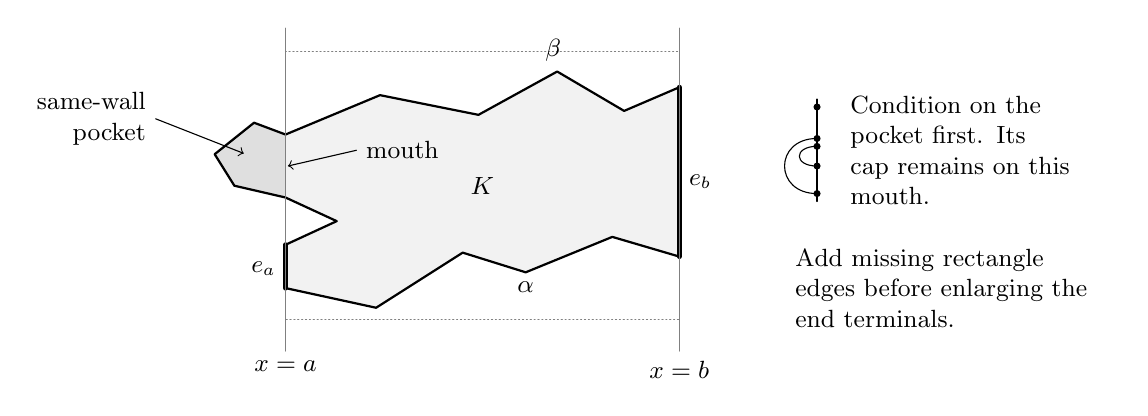
\begin{tikzpicture}[x=1cm,y=1cm,font=\small,line cap=round,line join=round]
  \draw[gray,densely dotted] (0,.25) rectangle (5,3.65);
  \path[fill=gray!10] (0,.65) -- (1.15,.4) -- (2.25,1.1) -- (3.05,.85) -- (4.15,1.3) -- (5,1.05)
    -- (5,3.2) -- (4.3,2.9) -- (3.45,3.4) -- (2.45,2.85) -- (1.2,3.1) -- (0,2.6)
    -- (0,1.8) -- (.65,1.5) -- (0,1.2) -- cycle;
  \path[fill=gray!25] (0,1.8) -- (-.65,1.95) -- (-.9,2.35) -- (-.4,2.75) -- (0,2.6) -- cycle;
  \draw[thick] (0,.65) -- (1.15,.4) -- (2.25,1.1) -- (3.05,.85) -- (4.15,1.3) -- (5,1.05);
  \draw[thick] (0,1.2) -- (.65,1.5) -- (0,1.8) -- (-.65,1.95) -- (-.9,2.35) -- (-.4,2.75)
    -- (0,2.6) -- (1.2,3.1) -- (2.45,2.85) -- (3.45,3.4) -- (4.3,2.9) -- (5,3.2);
  \draw[line width=1.8pt] (0,.65) -- (0,1.2);
  \draw[line width=1.8pt] (5,1.05) -- (5,3.2);
  \draw[densely dashed] (0,1.8) -- (0,2.6);
  \draw[gray] (0,-.15) -- (0,3.95);
  \draw[gray] (5,-.15) -- (5,3.95);
  \node[below] at (0,-.15) {$x=a$};
  \node[below] at (5,-.15) {$x=b$};
  \node[left] at (0,.9) {$e_a$};
  \node[right] at (5,2) {$e_b$};
  \node at (2.5,1.95) {$K$};
  \node[above] at (3.4,3.4) {$\beta$};
  \node[below] at (3.05,.85) {$\alpha$};
  \draw[<-] (-.53,2.36) -- (-1.65,2.8);
  \node[anchor=east,align=right] at (-1.65,2.8) {same-wall\\pocket};
  \draw[<-] (.03,2.2) -- (.9,2.4);
  \node[anchor=west] at (.9,2.4) {mouth};
  \draw (6.75,1.75) -- (6.75,3.05);
  \fill (6.75,1.85) circle (.045);
  \fill (6.75,2.2) circle (.045);
  \fill (6.75,2.45) circle (.045);
  \fill (6.75,2.55) circle (.045);
  \fill (6.75,2.95) circle (.045);
  \draw (6.75,1.85) .. controls (6.2,1.85) and (6.2,2.55) .. (6.75,2.55);
  \draw (6.75,2.2) .. controls (6.45,2.2) and (6.45,2.45) .. (6.75,2.45);
  \node[align=left,anchor=west,text width=3.2cm] at (7.05,2.4)
    {Condition on the pocket first. Its cap remains on this mouth.};
  \node[align=left,anchor=west,text width=4cm] at (6.35,.65)
    {Add missing rectangle edges before enlarging the end terminals.};
\end{tikzpicture}
\caption{A slab core cut from a winding corridor (schematic; lattice steps are suppressed). Consecutive opposite-wall cuts $e_a,e_b$ retain the ends. Same-wall excursions beyond a slab level are pockets, removed along their mouths to obtain $K$. Each pocket induces a separate noncrossing cap on its own mouth. The rectangle comparison preserves these caps while adding missing edges; only afterwards are the contact intervals merged with their respective terminals.}
\label{fig:slab-pockets}
\end{figure}


\smallskip\noindent
\emph{Good slabs and their cost.}
Fix a small number $\tau>0$, say $\tau=1/100$.  Choose $\zeta>0$
sufficiently small compared with $\tau^4$, and subsequently choose a
fixed integer $S_0$ sufficiently large compared with $\zeta^{-1}$ and
all lattice roundoff constants.  Take a maximizing collection for
$V_x$.  Its terms with $s<S_0$ cost at most $O(R^2S_0^4)$, which is
$O(R^4)$ with these fixed choices.  Group the remaining spans by
$h\le s<2h$, where $h=2^kS_0$.  Round the two end levels inward to a
common integer grid of spacing $\lfloor\zeta h\rfloor$, choosing
$a,b$ strictly inside them.  Each moves by at most $\zeta h+1$, so
\[
 b-a\ge s-O(\zeta h+1).
\]
Construct one $J,K,\alpha,\beta$ as above for each chosen passage.
Call it good if
\begin{equation}
 (p_+-p_-)+(P_+-P_-)
 +|\beta(a)_y-\alpha(a)_y|
 +|\beta(b)_y-\alpha(b)_y|\le\zeta h.
 \label{rect:good-slab}
\end{equation}

Members of the maximizing collection may share an end cut.  The chosen
levels $a,b$ lie strictly between each member's own end levels, so its
subquadrilateral $J$ does not use such a common end cut.  Their original
side-wall subarcs have disjoint longitudinal interiors.  Hence the
constructed core interiors are disjoint; any remaining boundary contact
only permits equality in the ordering below.
For a fixed pair $a,b$, the core disks are slab-ordered.  Their
bounding crossings cannot interleave: a slab crossing belonging to one
core would then separate points of the connected interior of another.
Minima, maxima, and the two endpoint heights of ordered disjoint
crossings are ordered as well, with weak inequalities sufficient.
Thus each of the four nonnegative gap sums in
\eqref{rect:good-slab} telescopes to at most $H$, and their total is at
most $4H$.  The number of bad choices at fixed $a,b$ is at most
$4H/(\zeta h)$.  There are $O_\zeta((R/h)^2)$ rounded pairs, so at this
scale there are $O_\zeta((R/h)^3)$ bad choices.  Their contribution to
$V_x$ is $O_\zeta(R^3h)$.  Summing over the dyadic scales $h\le R$
gives $O(R^4)$.

\smallskip\noindent
\emph{Amplification of a good passage.}
For a good passage the height $P_+-p_-$ is at least $b-a-O(1)$.
Otherwise the comparison rectangle \eqref{rect:comparison-box} would
be hard in the sense of \eqref{rect:hard-square}, contradicting the
connection probability at least $1-\epsilon$ in $J$.  Subtracting the
two extrema gaps in \eqref{rect:good-slab} gives the mandatory inner span
\begin{equation}
 T:=P_--p_+\ge s-O(\zeta h+1).
 \label{rect:inner-span}
\end{equation}
Choose integer levels a bounded distance inside $p_+$ and $P_-$.
Every end-to-end path visits both strict sides of each of these levels,
so the level-cut fact gives horizontal transversals.  The span between
two such low and high cuts is $T-O(1)$.

If $T\ge1.05s$, that one horizontal passage already has fourth power
larger than $(1+\gamma)s^4$ for some fixed $\gamma>0$, once $S_0$ is
large.  Otherwise the height and width of \eqref{rect:comparison-box}
are within the aspect-ratio range of Lemma~\ref{rect:corner}.  Every
point of each end interval must be at least $s/16$, for definiteness,
above the lower extreme and below the upper extreme, after increasing
$S_0$ and decreasing $\zeta$ if necessary.  Indeed if one endpoint
interval approaches an extreme more closely, the endpoint gap bound
in \eqref{rect:good-slab} places all contacts on that vertical side
within $s/16+O(\zeta h+1)$ of that extreme.  The comparison box then
has a corner electrode contained in its bottom or top eighth, and
Lemma~\ref{rect:corner} contradicts high connection.

Starting from the longitudinal first end of $J$, consider the earlier
of the selected low and high transversals.  The original end lies in
the central height range just established, while that earlier cut is
near the corresponding extreme.  Choose an intermediate horizontal
integer level between them at distance at least $\tau s$ from the
extreme cut.  The two ends of this first subquadrilateral are on strict
opposite sides of the intermediate level, so it contains a transversal
there.  The resulting extra horizontal passage precedes the low--high
passage and has disjoint longitudinal interior from it.  This works
in either order of the low and high cuts.  Its span is at least
$\tau s$, with bounded roundoff absorbed by the choices of constants.

The two contributions are therefore at least
\[
 \bigl(1-O(\zeta+S_0^{-1})\bigr)^4s^4+\tau^4s^4
 \ge(1+\gamma)s^4
\]
for a fixed $\gamma>0$, by choosing $\zeta$ and then $S_0^{-1}$ small
enough compared with $\tau^4$.  The constructed horizontal passages
are contained in their respective original vertical subquadrilaterals,
so all chosen contributions retain disjoint interiors.

\smallskip\noindent
\emph{Conclusion.}
Combining the good passages and the two error bounds gives
\[
 V_y\ge(1+\gamma)(V_x-C_0R^4).
\]
The same construction with the two coordinate directions exchanged,
and with the original longitudinal wall roles unchanged, gives
\[
 V_x\ge(1+\gamma)(V_y-C_0R^4).
\]
Substitution bounds each variation by a constant multiple of $R^4$.
Together with \eqref{rect:initial-variation}, this proves
\eqref{rect:packing-bound}.
\end{proof}

\subsection{Rectangle crossing bounds}

We now apply the packing lemma. The first half of the contradiction
argument concerns network probabilities in ordinary rectangles. The
second half puts finitely many primal and dual events in one law,
extracts actual crossings, and uses their unexplored sides to obtain
the pure corridor laws required by Lemma~\ref{rect:packing}.

\begin{proposition}[Rectangle RSW for separate electrodes]
\label{prop:rectangle-rsw}
For every fixed $\Lambda\ge1$ there is $c_\Lambda=c_\Lambda(q)>0$
such that
\begin{equation}
 \inf_{\substack{n,w\in\Z_{\ge1}\\w\le\Lambda n}}g_x(w,n)
 \ge c_\Lambda.
 \label{rect:rsw}
\end{equation}
The same holds after translation, lattice rotation, reflection, or
translation to the shifted dual square lattice.  All probabilities
refer to separate full crossing electrodes with no other wires.
\end{proposition}

\begin{proof}
Suppose otherwise.  Lemma~\ref{rect:square} and positivity on each
fixed finite graph give a sequence with
\begin{equation}
 n\longrightarrow\infty,\qquad n\le W_n\le\Lambda n,
 \qquad g_x(W_n,n)\longrightarrow0.
 \label{rect:degeneration}
\end{equation}
All limits in $n$ below are along \eqref{rect:degeneration}. Every
macroscopic separation, relative interval width, and bulk clearance
invoked in a convergence assertion is fixed and positive before taking
that limit. These constants may depend
on the finite number of chords to be used, but not on $n$. A convergence
assertion for a stated class of rectangles and intervals means that it
holds for every sequence of integer choices satisfying those same fixed
conditions. Equivalently, the convergence is uniform over that class:
a failure of uniformity would select a violating sequence, to which
the same subsequence contradiction applies.

\smallskip\noindent
\emph{Separated arches vanish.}
For each fixed $\sigma>0$, consider ordinary rectangles with positive
integer width and height at most $n/8$, and two nonempty top intervals
whose horizontal separation is at least $\sigma n$. Their network
probability tends to zero uniformly over these choices. Otherwise, after taking a
subsequence, there is such a chord bounded below.  Subdivide both
intervals into a bounded number of subintervals of diameter at most
$\sigma n/10+O(1)$.  By \eqref{rect:subadditivity}, a pair of these localized
intervals still has a chord bounded below.  Translate copies of its
rectangle along the top of $R_{W_n,n}$, starting at the left side, with
integer displacement close to half the separation of the two localized
centers.  Consecutive chords interlace strictly; they retain their lower
bounds by Lemma~\ref{rect:extension}.  Continue while the rectangles
fit.  A bounded number of applications of
\eqref{rect:interlacing}, depending only on $\sigma,\Lambda$, joins the
first endpoint to the last far endpoint with probability bounded below.
The first lies within $n/8$ of the left side and the last within
$n/8+n/16+O(1)$ of the right side.

A square of side $\lfloor n/2\rfloor$ at the upper-left corner has a
chord from its left side to the far half of its top side bounded below:
reflection and subadditivity give the half-side crossing, then
interlacing with an opposite full square crossing gives the stated
chord.  The analogous upper-right square gives the other end chord.
They interlace the long top chord to the full left and right sides.
This contradicts \eqref{rect:degeneration}.  Reflection gives the same
vanishing statement for bottom arches.  Translation gives it on the
shifted grid as well.

\smallskip\noindent
\emph{Only aligned chords can survive.}
Fix $0<c_-\le c_+\le1/8$ and $0<\theta<1/2$. For integer square sides
$c_-n\le h\le c_+n$, a top electrode contained in
$[0,(1/2-\theta)h]$ or in $[(1/2+\theta)h,h]$ connects to the full
bottom side with probability tending uniformly to zero.
If not, reflect that electrode and its chord across the vertical center
line.  Interlace the two top--bottom chords separately with the
full left--right square crossing, whose probability is bounded below.
This yields chords from the left top portion to the right side and
from the right top portion to the left side.  Interlacing them gives
a separated same-top arch, contradicting the preceding paragraph.
The corresponding off-center bottom chords also vanish.

Decompose each of the top and bottom sides into its two off-center
portions and the central interval
$[(1/2-\theta)h,(1/2+\theta)h]$, with endpoints rounded to lattice
vertices. The full
vertical crossing has a uniform lower bound.  Subadditivity twice,
and the vanishing just proved, therefore give a positive lower bound
for the chord between the two central neighborhoods.

Now use an integer strip of height $h$ and width $\ell=4h+O(1)$, with
the bound in $O(1)$ fixed,
$h/n$ bounded above and below by fixed positive constants and both
dimensions at most $n/8$. Translated squares give bounded-below chords
between aligned top and bottom patches of fixed positive relative width.
Their centers may vary provided their distances from the vertical ends
are at least $(1/2+\eta)h$ for a fixed $\eta>0$.

In this strip, consider boundary electrodes lying entirely to the left
and right, respectively, of a horizontal gap. Suppose that the gap
contains centers $c_1<c_2$ whose distances from its endpoints and from
each other are at least $\eta h$, and whose distances from the vertical
strip ends are at least $(1/2+\eta)h$, for some fixed $\eta>0$.
The connection probability of those electrodes tends uniformly to zero.
Choose the aligned patches at these centers with length
$\eta h/2+O(1)$ after lattice rounding, so that the two patches are disjoint and
remain in the gap. Interlace a hypothetical
bounded-below chord with the aligned vertical chord at the first
center, joining that top patch to the right electrode, and with the
aligned chord at the second center, joining that top patch to the left
electrode.  The resulting chords interlace to give a forbidden
separated same-top arch.

\smallskip\noindent
\emph{Aligned short electrodes are crossed with probability tending
to one.}
Fix $\theta,\eta>0$ and equal aligned intervals on the top and bottom
of this strip, each of length at least $\theta h$ and contained between
horizontal coordinates $(1/2+\eta)h$ and $\ell-(1/2+\eta)h$.
Contract their boundary edges.
The complementary dual crossing is between the exterior arcs going
around the left and right ends.  Split the corresponding exterior
hub into two hubs.  This costs only a bounded density factor.  Absorb
all adjacent contact vertices into their respective hubs, which cannot
decrease the network probability by terminal monotonicity. The result is an
ordinary interior cell rectangle with two separately wired boundary
electrodes whose horizontal coordinates are separated by the gap
between the endpoints of the original intervals. This gap contains
two centers satisfying the preceding fixed-clearance conditions, with
constants depending only on $\theta,\eta$. The preceding vanishing
argument, on the shifted grid and with bounded lattice roundoff,
applies to this network.  Thus the complementary dual probability
tends to zero, and the original aligned crossing tends to one.
Smaller aligned subintervals of any fixed positive relative width are
covered by the same argument.

\smallskip\noindent
\emph{Many alternating network crossings.}
The preceding steps have shown that every fixed aligned pair of short
intervals in the indicated strip is crossed with probability tending
to one. We next arrange finitely many such primal and dual crossings
in a common law. Their simultaneous success will use a union bound;
no correlation inequality between these events is needed.

For definiteness take $h=\lfloor n/64\rfloor$ and strip width $4h$.
Choose an arbitrarily large but fixed finite ordered list of disjoint
small interval labels in a central bulk part of the top side, and
matching labels in the same order on the bottom.  On the primal graph
wire the odd intervals, each separately, by contracting their boundary
edge runs.  Leave no other primal wires.  Round the runs so that each
intervening even interval retains an uncontracted boundary-edge stretch
of fixed positive relative width.  Only interior labels with neighboring
buffers will be used.

Every desired odd top--bottom network connection tends to one.  This
follows first in the pure two-electrode graph by the aligned estimate,
then in the multiwire graph by adding the other disjoint interval caps
cofacially with its test edge.  The deletion order is the exposed
boundary face expansion used in Lemma~\ref{rect:extension}.

The dual consists of the cell grid and a common outer hub with
stochastic spokes dual to all uncontracted boundary edges.  Split this
hub into separate hubs for the maximal complementary intervals.  Since
the number of intervals is fixed, the density change is bounded by a
fixed power of $q^{-1}$.  We claim that each desired even top--bottom
connection in this split network also tends to one, despite the finite
spoke odds.

Retain first only the two spoke patches over smaller aligned intervals.
Fix a deterministic bottom subinterval wire in that range.  For any
fixed integer $k$, choose $k$ disjoint smaller top patches aligned
within it.  Each is connected to the bottom wire with probability
tending to one by the pure estimate and terminal enlargement.  In the
single rooted-multiset law based at the collapsed bottom electrode,
all $k$ patches are therefore hit with probability tending to one.
Their union has multiplicity at least $k$ on that event.  Formula
\eqref{rect:spokes} gives lower limit at least $1-(1+v)^{-k}$ for the
finite top-spoke connection.  Since $k$ is arbitrary, this probability
tends to one.  Now keep this finite top-spoke graph as the base rooted
at its hub.  Apply the same argument to $k$ disjoint deterministic
bottom subintervals, using the conclusion just established for each
of them.  This makes the bottom spokes finite as well, still with
connection tending to one.  The order of limits is first $n\to\infty$
for fixed $k$, then $k\to\infty$.

Extra spokes at the tested hubs cannot decrease connection.  Spokes of
each other hub occupy its own exposed boundary interval and can be
removed by exterior face expansion from the test-edge faces; reversing
this removal does not decrease the tested connection.  Thus the desired even
events tend to one in the full split dual network.  The bounded
hub-joining density transfers them back to the common original law.
Their event definition still uses only the individual split-hub
shortcuts, not the common hub as a path shortcut.

\smallskip\noindent
\emph{From networks to physical crossings.}
All these finitely many primal and dual successes coexist with
probability tending to one.  Draw shortcuts narrowly along their
separate boundary intervals, including dual spokes through the
appropriate boundary-edge midpoints.  Complementary primal and dual
states prevent crossings of opposite-color open paths. For topology
only, place the rectangle and all narrow caps inside a slightly enlarged
disk, and join each designated terminal to a distinct point on its
boundary by outward spokes, preserving the order of the terminal intervals.
For a dual event, the shortcuts here are those of its individual
split hubs, although its edge state is now sampled in the common law.

For each network success, choose a simple witness in this enlarged
disk, with the narrow cap shortcuts included as edges. Its only
contacts with the enlarged boundary are its prescribed top and bottom
endpoints, so it is a crosscut even if it uses another same-color cap
along the way. Opposite-color witnesses are disjoint: their physical
edges cannot cross, and their cap shortcuts and outward spokes occupy
disjoint boundary intervals.

Fix a successful interior label whose two opposite-color neighbors
also succeed. The target crosscut places the endpoints of one neighbor
on one side and those of the other neighbor on the other side.
Their witnesses cannot cross the target, so they lie on those
respective sides and are disjoint from each other. The region between
them meets the top and bottom boundary exactly between the neighboring
labels. Every other same-color cap lies outside that region: its narrow
connection to its own boundary interval is disjoint from the two
neighbors. The target witness therefore cannot use another same-color
wire or hub. Its segment from the last departure from its initial
terminal to the first subsequent arrival at its final terminal is therefore an
actual physical crossing between its labeled intervals.
For a dual label, the crossing retains its initial and final stochastic
boundary spokes and an ordinary cell path, with no intermediate hub
jump. This proves simultaneous physical success for the slightly
smaller range of interior labels that has all required buffers.

\smallskip\noindent
\emph{Uninspected high corridors.}
Select many odd interior labels spaced by at least four.  For each
selected $i$, expose a physical dual crossing for label $i-1$ from
its left side, and one for label $i+1$ from its right side.  The
search uses the physical cell graph with its available boundary
half-extensions at that pair of intervals and fictitious always-open
terminal stars confined to their outer caps. Seed the complementary-face
search at the corresponding exterior side. Query an edge only from a reached face, and advance to the
opposite face only when its physical bond in the path color is closed.
On crossing success this exploration stays outside
every blocking terminal path.  Setting all unqueried edges to the
nonpath state still leaves a path, by the plane path--cut alternative,
so choose a simple witness measurably from the exposed edges.  No
edge with interior on its other side was queried.  The ordered
boundary spokes preserve this property at the endpoints.  Stop each
wall at the physical rectangle boundary-edge midpoint.

Let $\mathcal R_i$ be the combined record of the two searches, including
the queried edge states and the chosen walls. Let $E_i$ be the event,
determined by this record, that both searches succeed with disjoint
walls in the proper order. The simultaneous physical crossings,
including the odd target path separating its two neighbors, imply
$\PP(E_i)\to1$.

Fix a value of $\mathcal R_i$ in $E_i$. Every fully contained primal
edge between the walls, other than the deterministic boundary edges
along the target wires, is uninspected, and every primal edge crossing
a wall is closed. The top and bottom intervals contain exactly the
two target primal wires: the wall endpoints lie in the flanking
uncontracted intervals, and no exterior tie enters the corridor.
Omit the boundary edges along the target wires, which are independent
loops after contraction, and let $G_i$ be the remaining contained-edge
graph. Finite conditioning now gives exactly the FK law on $G_i$ with
the two target electrodes separately wired. Indeed the queried closed
edges separate the corridor from the exterior across both walls, and
the original boundary partition has
no other class meeting the corridor; integrating the exterior therefore
introduces no additional identification. Restoring the omitted loops
with their independent ordinary law changes no crossing probability.

Let $g_i$ be the pure corridor probability from
Definition~\ref{rect:corridor-definition}, measurable from
$\mathcal R_i$, and let $T_i$ be the target's actual physical crossing
event in the original strip. On $E_i$, such a path cannot cross either
dual wall, so it is contained in the corridor. The preceding conditional
law and the two-wire path equivalence give
$\PP(T_i\mid\mathcal R_i)=g_i$ on $E_i$. Since $\PP(T_i)\to1$,
\begin{equation}
 \EE\bigl[(1-g_i)\one_{E_i}\bigr]
   =\PP(E_i\cap T_i^c)\longrightarrow0.
 \label{rect:conditional-high}
\end{equation}
Markov's inequality gives $g_i\ge1-\epsilon$ on $E_i$ with probability
tending to one.  Perform these searches on the same configuration for
each of the finitely many selected indices.  Equation
\eqref{rect:conditional-high} was applied separately to each search;
no joint unexplored independence is required.  With probability tending
to one all the high-corridor conclusions hold together with the
intervening physical crossings.  In particular intervening odd primal
crossings separate different pairs of dual walls, so the resulting
corridors have disjoint closures.

The strip aspect ratio is fixed.  Choose the finite number of selected
labels larger than the constant allowed by
Lemma~\ref{rect:packing}.  For large $n$, any realization with all the
preceding properties violates \eqref{rect:packing-bound}.  Such
realizations have probability tending to one, a contradiction.  This
proves \eqref{rect:rsw}.
\end{proof}

\subsection{One-sided boundary density}

The rectangle crossing bound is now proved. For the later sector and
disk arguments we also need to control partition-function gains when
a distant boundary wire is changed. These comparisons use
Section~\ref{sec:pressure} directly, independently of the rectangle
crossing proposition. We return to arbitrary positive
edge odds on a finite ordinary plane graph $H$ in a closed disk, with
no initial wires. Lemma~\ref{lem:one-sided-density} bounds that interaction
by the pure connection probability; the final subsection replaces full
wires by arbitrary separate planar caps.
For a nonempty vertex set $D$, let $k_D$ count physical open components
meeting $D$, and put
\[
 K_H(D)=\log\EE_H t^{k_D},\qquad
 \Delta_H(S,W)=K_H(S)+K_H(W)-K_H(S\cup W).
\]
The coverage representation from Lemma~\ref{lem:rooted} gives
$\Delta_H(S,W)\ge0$.  Denote the full wire on $D$ by $F_D$.
For a partition $X$ let $Z_X$ be the partition function on the original
edge sets with weight $v_Aq^{k_{H/X}(A)}$, retaining any quotient loops;
write $Z=Z_\varnothing$.

\begin{lemma}[Auxiliary-link gain in an exposed face]
\label{rect:face-gain}
Let $e$ be a physical edge bordering a face $F$ of a finite plane
graph.  Let $T$ be a finite noncrossing collection of auxiliary links
whose endpoints are graph vertices and whose interiors lie in $F$.
At fixed positive auxiliary odds, the partition-function gain from
adding all links of $T$ is nonincreasing in the odds of $e$.
The conclusion passes to a prescribed partition obtained by contracting
the links.  Repeated boundary vertices, auxiliary loops, and redundant
links are allowed in the corresponding plane minors.
\end{lemma}

\begin{proof}
In the drawing with all links present, start from a face sector incident
to $e$.  The dual adjacency graph of regions into which the links cut
$F$ is connected, since the original face $F$ was connected.  Remove
a frontier auxiliary link to expand the reached $e$-face and repeat,
also removing auxiliary links with that reached face on both sides.
Eventually every link is removed.  Reverse this order.  At each
addition, the link and $e$ are cofacial in the graph including the new
link.  Cofacial Rayleigh implies that its log partition gain, integrated
from zero to its specified odds, is nonincreasing in the odds of $e$.
Sum these log gains.  The removal order may be chosen separately for
each physical edge and each background graph.

For auxiliary odds $\lambda_f$, divide the augmented partition function
by $\prod_{f\in T}\lambda_f$ and send every $\lambda_f$ to infinity.
Only the term with all auxiliary links open survives, and it is exactly
the contracted-graph partition function.  Retaining the same links and
normalizing product after any physical minor handles links that become
loops or redundant.  This proves the limit statement as well.
\end{proof}

\begin{lemma}[One-sided small-network density]
\label{lem:one-sided-density}
Let $S,W$ be disjoint nonempty vertex sets on two disjoint accessible
boundary arcs of $H$.  Put $p=g_H(S,W)$ and suppose $tp<1$.
For every noncrossing partition $X$ supported on $S$,
\begin{equation}
 0\le \log\frac{Z_XZ_{F_W}}{Z_{X,F_W}Z}
 \le\Delta_H(S,W)
 \le\log\left(1+\frac{(t-1)p}{1-tp}\right).
 \label{rect:one-sided-density}
\end{equation}
\end{lemma}

\begin{proof}
There are three steps. A component exploration bounds the number of
physical crossings by a geometric tail. A covariance inequality turns
that tail into the asserted upper bound on $\Delta_H(S,W)$. Finally,
an exact full-wire identity and cofacial comparison give the two bounds
for an arbitrary partition $X$.

\paragraph{A geometric tail for crossing components.}
In either the separately
$S,W$-wired law or their jointly wired law, let $L$ be the number of
distinct physical components meeting both sets, before any identification.
Then
\begin{equation}
 \PP(L\ge j)\le p^j\qquad(j\ge1).
 \label{rect:component-tail}
\end{equation}

Explore whole physical components from the vertices of $W$ in their
linear boundary order, skipping vertices already visited and never
following a wire as a physical edge.  Component searches test every
incident physical edge.  After a prefix, possibly stopped immediately
after a crossing component, let $U$ be the explored union.  Every
vertex of $U$ has a path in $U$ to that prefix.  On $H-U$, component
counting leaves precisely the full remaining $W$ and $S$ wires,
possibly joined, and no other ties.  Joining them multiplies the
weight of separation by $t$ relative to connection; hence the
conditional probability of another crossing component is at most
\[
 g_{H-U}(W\setminus U,S\setminus U),
\]
interpreted as zero if either set is empty.

This last quantity is at most $p$.  To verify the comparison rather
than invoke arbitrary boundary monotonicity, keep all vertices of $H$
temporarily.  Draw narrow exterior chains along $W$ and $S$, and a
test edge from the first $W$ vertex to the facing endpoint of $S$
across the intervening gap.  Starting in its gap-side face, delete
the physical fan of the first $W$ vertex.  This opens the inner lip
of the narrowly exterior chain up to the next prefix vertex.  The
thin sector between a chain link and its underlying boundary interval
contains no physical edge or other auxiliary link, so the exposed
face can advance successively along the entire explored prefix.
Continue into $U$ along paths to that prefix: deleting an onward
physical edge exposes a sector at the next vertex, from which its
whole physical fan can be deleted in order.  At a boundary vertex
the physical fan is inward and contains no interspersed auxiliary
links.  No chain link needs to be removed.  Thus every removed
physical edge is cofacial with the test edge at its removal.

At finite positive chain odds, cofacial Rayleigh makes connection
nonincreasing under these deletions.  Send the chain odds to infinity.
This comparison starts from the original \emph{separate}-wire graph,
not from the conditional graph in which a previous crossing may have
joined the electrodes.  Every physical edge touching $U$ has been
deleted, and the retained $W$ and $S$ chains have disjoint vertex sets;
they cannot create a tie between the two sides.  After contracting
each chain, a test endpoint originally in $U$ is the same quotient
vertex as any surviving vertex of its own electrode.  Use such
surviving representatives on both sides; the case of an empty surviving
electrode was already assigned probability zero.  Isolated vertices
off the two chains factor out.  Thus the remaining test is exactly the
separate two-electrode problem on $H-U$, irrespective of whether the
earlier conditional problem had joined wires.
This proves the comparison.  Each successive exploration success
therefore has conditional probability at most $p$, and iteration
proves \eqref{rect:component-tail}, including for the initially
joined law.

\paragraph{From the tail to the full-wire interaction.}
We need the rank-factor covariance inequality
\begin{equation}
 \EE_H t^{k_S+k_W}\ge
 \EE_H t^{k_S}\,\EE_H t^{k_W}.
 \label{rect:rank-covariance}
\end{equation}
Here is its finite-graph proof.  More generally consider two full-wire
rank factors $t^{k_D-1}$, where each set can be joined by links inside
one common physical face; the two prospective drawings may be
considered separately.  The invariant under minors is the inherited
auxiliary drawings in one common physical face, not the original
disjoint-arc description: image electrodes may overlap or shrink.
Induct on the number of physical edges.
Choose an edge $e$ bordering that face.  For either prospective wire,
its expected rank factor conditional on $e$ open is no greater than
conditional on $e$ closed.  Draw its auxiliary links at finite odds,
peel them from a face sector incident to $e$, and add them back in
reverse order.  At each addition the new link and $e$ are cofacial in
the graph containing both, as in Lemma~\ref{rect:face-gain}.
Cofacial Rayleigh says that its
partition-function gain is nonincreasing with the odds of $e$.
Multiply these gains and take the full-wire limit.  This proves the
asserted conditional-mean inequality.

In each of deletion and contraction of a nonloop $e$, the prospective
wire drawings remain in the image of the same face.  The rank factors
restrict exactly to the corresponding rank factors of the minor,
with coincident marked vertices identified.  Thus the conditional
covariances are nonnegative by induction.  The additional term in
the total-covariance formula is nonnegative because both conditional
mean differences have the same sign.  A loop changes neither rank
factor and can be omitted; if no physical edge remains, the factors
are deterministic.  This completes the induction.  To take an
auxiliary-wire limit without ambiguity, divide the augmented
partition function by the product of all auxiliary odds before
sending them to infinity.  The surviving all-open term is exactly
the contracted-graph partition function, even when some links have
become redundant or loops in a minor.  Since $S,W$ are on the same
outer face, the general inequality yields
\eqref{rect:rank-covariance}.

Every physical component meeting both $S,W$ is counted twice on the
left and once on the union, so
$L=k_S+k_W-k_{S\cup W}$.  Equation
\eqref{rect:rank-covariance} therefore gives
\begin{equation}
 e^{\Delta_H(S,W)}
 \le\frac{\EE_H t^{k_S+k_W}}{\EE_H t^{k_{S\cup W}}}
 =\EE_{H/F_{S\cup W}}t^L.
 \label{rect:interaction-moment}
\end{equation}
The normalization for full wiring is $t^{k_{S\cup W}-1}$; its
constant factor cancels in this expectation.  From
\eqref{rect:component-tail},
\[
 \EE t^L
 =1+(t-1)\sum_{j\ge1}t^{j-1}\PP(L\ge j)
 \le1+\frac{(t-1)p}{1-tp}.
\]
This proves the final upper bound in
\eqref{rect:one-sided-density}.

\paragraph{An arbitrary partition on the first end.}
Let $S'$ be the image of $S$ in $H/X$.  A full-$D$ log gain is
$K_H(D)-\log t$, and the full $S$ and full $S\cup W$ wires both
subsume $X$.  Writing these gains out gives the exact identity
\begin{equation}
 \log\frac{Z_XZ_{F_W}}{Z_{X,F_W}Z}
 =\Delta_H(S,W)-\Delta_{H/X}(S',W).
 \label{rect:interaction-difference}
\end{equation}
Coverage positivity in the quotient proves the middle upper bound.

For the lower bound draw the noncrossing $X$ links and a full-$W$
chain in separate exterior caps facing the main exterior.  Peel the
$X$ links from that main face and add them in reverse order.  For
each link being added, the $W$ links may likewise be ordered by
reverse peeling from its incident outer-face sector.  Each compared
pair is then cofacial at the moment of comparison.  Cofacial Rayleigh
does not increase the $W$ partition gain when the $X$ links are present.
Integrate at finite odds, multiply the successive gains, and take
the wire limits with the preceding normalization.  Thus
$Z_{X,F_W}/Z_X\le Z_{F_W}/Z$, proving nonnegativity and completing
the lemma.
\end{proof}

\begin{corollary}[A marginal comparison]
\label{rect:one-sided-marginal}
Suppose that an exterior configuration meets a collar only along $S$
and induces there an arbitrary noncrossing partition $X$, while $W$
is free.  If the collar's pure probability $g_H(S,W)$ tends to zero,
adding the full wire at $W$ changes the exterior marginal by a density
tending uniformly to one.
\end{corollary}

\begin{proof}
Conditional component counting makes the unnormalized density factor
$Z_{X,F_W}/Z_X$.  By Lemma~\ref{lem:one-sided-density} its ratio to
the fixed factor $Z_{F_W}/Z$ lies between $e^{-\varepsilon_p}$ and
one, where $\varepsilon_p\to0$.  Division by its average gives a
normalized density between $e^{-\varepsilon_p}$ and
$e^{\varepsilon_p}$, uniformly in $X$.
\end{proof}

\subsection{No-hit comparison and arbitrary separate caps}

The next result uses actual physical components throughout.  Neither
the event being compared nor its exploration is allowed to traverse a
boundary identification as a path edge.

\begin{lemma}[End-cap no-hit comparison]
\label{lem:no-hit}
Let $H$ be an ordinary finite plane graph in a closed disk, with
nonempty vertex sets $W,S$ on disjoint accessible boundary arcs and
no preexisting ties.  Let $X$ be a noncrossing partition on $W$ and
$Y$ one on $S$.  Adding $Y$ to the $X$-law does not increase the probability
of an actual physical $W$--$S$ crossing.  Adding $X$ alone to the
blank law also does not increase that probability.
\end{lemma}

\begin{proof}
Relative to the $X$-law, the extra partition gain is the nonnegative
random weight
\[
 f(A)=q^{k_{H/(X,Y)}(A)-k_{H/X}(A)},
 \qquad \EE_{H/X}f=\frac{Z_{X,Y}}{Z_X}.
\]
On no actual crossing, explore all complete physical open components
touching $W$, without using ties as physical links.  Their union $U$
contains $W$ and avoids $S$.  All edges from $U$ to its complement
are closed.  Every $X$ tie is contained in $U$, and conditional
component counting shows that the conditional mean of $f$ is exactly
the $Y$-partition gain in the ordinary graph $H-U$.

This gain is at least the unconditional mean of $f$ in the $X$-law.
Draw all prospective cap links.  With $Y$ temporarily absent in
describing faces, delete the $X$ links in an order expanding the
exterior face from the $S$ cap.  Then peel all physical edges touching
$U$ from this exposed face: start at $W$, delete its inward fans, and
continue along paths in each explored component to the vertices
reached.  All those components touch $W$, and no $S$ vertex is removed.
At each deleted edge $e$, the $Y$ log partition gain cannot decrease.
For a precise finite-odds comparison, peel the prospective $Y$ links
from the face sector incident to $e$ through their cap, then add them
in reverse order.  Each newly added link is cofacial with $e$ in
the graph containing both.  Cofacial Rayleigh makes its log gain
nonincreasing with the odds of $e$.  Decrease those odds to zero and
repeat.  The order for $Y$ may be chosen anew for each deleted edge;
there is no claim that all nested cap links are simultaneously
cofacial.  Finally send auxiliary odds to infinity after dividing
out their common leading product.  During physical peeling retain
the vertices of $U$ temporarily.  Since $U$ avoids all $Y$ endpoints,
its isolated vertices contribute the same factor $q^{|U|}$ to the
ordinary gain's numerator and denominator and then cancel.  This proves
the asserted comparison with
$H-U$.

Consequently
\[
 \EE_{H/X}[f\mid\text{no hit}]\ge\EE_{H/X}f.
\]
Tilting by $f$ does not decrease the no-hit probability, and hence does not increase
the physical crossing probability.  To compare the $X$-law with
the blank law, use the same argument with the two ends exchanged
and with the initial partition empty.
\end{proof}

\begin{lemma}[Decoupling of separate cap gains]
\label{lem:separate-caps}
In the setting of Lemma~\ref{lem:no-hit}, put
$b_H=\PP_H(W\leftrightarrow S)$ for the actual crossing probability
in the blank law.  Then
\begin{equation}
 (1-b_H)\frac{Z_Y}{Z}
 \le\frac{Z_{X,Y}}{Z_X}
 \le\frac{Z_Y}{Z}.
 \label{rect:separate-cap-gains}
\end{equation}
In particular, when $b_H\to0$, the gain of an arbitrary partition on
one end is asymptotically unchanged, uniformly, by an arbitrary
noncrossing partition on the other end.
\end{lemma}

\begin{proof}
The upper bound is the finite-odds cofacial cap comparison used at
the end of Lemma~\ref{lem:one-sided-density}, now with arbitrary
noncrossing $Y$ in place of a full wire.  Peel the cap links from
the main exterior and add them in reverse order, ordering the
opposite cap as necessary for each comparison.  Each pair is
cofacial when Rayleigh is applied.  Integrating and taking the
normalized contraction limits gives the upper bound.

For the lower bound, use the no-hit component exploration from
Lemma~\ref{lem:no-hit} in the $X$-law.  On no actual hit its
conditional $Y$ gain is the blank $Y$ gain in $H-U$.  By just the
physical-edge peeling part of that proof, comparing this time
against the empty base cap, that gain is at least $Z_Y/Z$.
Lemma~\ref{lem:no-hit} gives no-hit probability at least $1-b_H$.
Keeping only this nonnegative contribution to the mean of $f$ yields
\[
 \frac{Z_{X,Y}}{Z_X}=\EE_{H/X}f
 \ge\PP_{H/X}(\text{no hit})\frac{Z_Y}{Z}
 \ge(1-b_H)\frac{Z_Y}{Z}.
\]
This is the claimed inequality.
\end{proof}

\begin{remark}[Scope of the comparisons]
\label{rect:scope}
The two density statements require separate accessible end arcs with
all physical incidences on the disk side.  The last two lemmas start
with no obstructing preexisting ties.  Neither their proofs nor
Proposition~\ref{prop:rectangle-rsw} assert stochastic monotonicity
for arbitrary boundary conditions, or comparison between arbitrary
partitions on noncofacial rims.  These restrictions will be retained
when the estimates are used in more complicated domains.
\end{remark}
